\documentclass[10pt]{scrreprt}
\usepackage[a4paper, top=30mm, left=25mm, right=25mm, bottom=30mm]{geometry}
\usepackage[utf8]{inputenc}

%Options: Sonny, Lenny, Glenn, Conny, Rejne, Bjarne, Bjornstrup
\usepackage[Bjornstrup]{fncychap}
\usepackage{ngerman}
\usepackage{graphicx}
\usepackage{epstopdf}
\usepackage{etoolbox}
\usepackage{enumitem}
\usepackage{url}
\usepackage{numprint}
\usepackage{tabularx}

\makeatletter
\patchcmd{\@makechapterhead}{\vspace*{50\p@}}{\vspace*{-20\p@}}{}{}
\patchcmd{\@makeschapterhead}{\vspace*{50\p@}}{\vspace*{-20\p@}}{}{}
\makeatother


\begin{document}

\thispagestyle{empty}
\sffamily
 
\title{Pflichtenheft}

\begin{figure}
\begin{flushright}
	
\includegraphics[scale=0.4]{uniLogo.eps}
\vspace{2.0 cm}
\end{flushright}
\end{figure}

\begin{center}
\vspace{2.0 cm}
{\LARGE SEP – Wintersemester 2013/14}

\vspace{1.0 cm}
\textbf{{\Huge Pflichtenheft}}

\vspace{0.8 cm}
\begin{figure}[!htb]
\begin{center}
	%
\includegraphics[scale=1.0]{projektLogo.eps}
	
\includegraphics[scale=1.5]{Logo-Print.eps}
\end{center}
\end{figure}

\vspace{0.2 cm}
\textbf{{\huge OpenStreetMap: Die Welt in 3D}}

\vspace{1.5 cm}
[endgültiges Datum]

\vspace{0.5 cm}
Version: 1.0

\vspace{1.5 cm}
{\Large Projektbetreuer: Peter Barth}

\vspace{1.5 cm}
\begin{tabular}{|c|c|c|}
\hline 
\rule[-1ex]{0pt}{4ex} \textbf{Phase} & \textbf{Verantwortlicher} & \textbf{E-Mail Adresse} \\ 
\hline  \hline
\rule[-1ex]{0pt}{4ex} Pflichtenheft & Gabriele Haas & haasgab@fim.uni-passau.de \\ 
\hline  \hline
\rule[-1ex]{0pt}{4ex} Entwurf & Thomas Eder & ederthom@fim.uni-passau.de \\ 
\hline  \hline
\rule[-1ex]{0pt}{4ex} Spezifikation & Christof Blauberger & blauberg@fim.uni-passau.de \\ 
\hline  \hline
\rule[-1ex]{0pt}{4ex} Implementierung & Fabian Knorr & knorrfab@fim.uni-passau.de \\ 
\hline \hline 
\rule[-1ex]{0pt}{4ex} Testing & Constantin Wenger & wengerco@fim.uni-passau.de \\ 
\hline  \hline
\rule[-1ex]{0pt}{4ex} Präsentation & Sebastian Reichl & reichlse@fim.uni-passau.de \\ 
\hline 
\end{tabular}

\end{center}



\rmfamily
\tableofcontents



\chapter{Ausgangssituation}
Die Kartendaten des OpenStreetMap-Projekts erfreuen sich immer größerer Beliebtheit. Der Detailgrad der Daten, die Menge an verschiedenen Merkmalen und die Genauigkeit der Daten sind in den meisten Regionen der Welt ihrer Konkurrenz weit voraus. Durch die verschiedenartigen Karten, Kartenstile und Spezialanwendungen auf Basis von OpenStreetMap gibt es eine unzählige Menge von Anwendungsmöglichkeiten.

Außerdem ist die Grafikleistung einfacher Desktoprechner bereits für aufwändige 3D-Anwendungen ausgelegt. Die Vorlieben der Benutzer hat sich in den letzten Jahren dahingehend geändert, dass die visuelle Gestaltung wie auch die intuitive Bedienung ausschlaggebend für die Wahl eines Softwareproduktes ist.

\vspace{0.5cm}

Zwar existieren bereits ähnliche Softwarepakete, jedoch keines mit den folgenden Schwerpunkten:
\begin{itemize}
\item Primäre Verwendung von Kartendaten des OpenStreetMap-Projekts
\item Freie Wählbarkeit von Kartenquellen durch den Benutzer
\item Intuitive Bedienung ohne Einarbeitungszeit
\item Die Möglichkeit der spielerischen Benutzung durch Kinder ohne PC-Kenntnisse
\item Vollständige Plattformunabhängigkeit durch Java
\item Effiziente Speicher- und Bandbreitennutzung
\end{itemize}

\vspace{0.5cm}

Mit diesen Grundprinzipien soll eine 3D-Desktopanwendung basierend auf den Daten von OpenStreetMap und der NASA entworfen werden.




\chapter{Produkteinsatz}
\section{Anwendungsbereich}
Die Desktopanwendung „Jogl Earth“ soll eine interaktive, dreidimensionale Ansicht der Welt auf Basis der freien Daten des OpenStreetMap-Projekt bieten. \\

Die grafische Benutzeroberfläche zeigt dafür eine Weltkugel, die frei gedreht und gezoomt werden kann. Die Steuerung erfolgt hierbei mit Tastatur und Maus. Die Oberflächentextur kann hierbei aus verschiedenen Typen wie Satellitenbildern der NASA oder Kartendaten des OpenStreetMap-Projekts gewählt werden. 
So besteht die Möglichkeit bis zu Straßenkarten zu zoomen und auch Städte oder andere Orte mit Hilfe einer Suchfunktion zu finden. \\

Es können auch weitere Anzeigeeinstellungen vorgenommen werden, wie eine freie Konfigurierbarkeit der Kartenserver oder das Einblenden von Overlays z.B. Banken, Tankstellen, Tierparks.  
Damit ist eine Anpassung der angezeigten Inhalte auf verschiedene Altersstufen und Interessengruppen möglich.


\section{Zielgruppe}
Primäre Zielgruppe des Systems sind Privatanwender, die eine andere Art der Kartendarstellung als die typischen Onlinekarten bevorzugen.

Eine weitere Zielgruppe sollen wissbegierige Kinder darstellen. Voraussetzung ist lediglich der geübte Umgang mit der Maus und/ oder Tastatur. (Eingeschränkte Features)

\section{Betriebsbedingungen}
\begin{itemize}
\item Bestehende dauerhafte Internetverbindung zum Laden des Kartenmaterials.
\item Nach der Abschlusspräsentation werden keine weiteren 
Veränderungen vorgenommen. Es erfolgt keine Wartung.
\end{itemize} 

\section{Sicherheit, Datenschutz}
Die Anwendung wahrt per Design die Sicherheit des Systems und schützt die Privatsphäre des Nutzers, da
\begin{itemize}
\item weder zur Bedienung, noch zum Beschaffen der Kartendaten eine Authentifikation erforderlich ist
\item keine Persönlichen Daten des Anwenders über das Netz übertragen werden
\item nie ein aus dem Netz nachgeladener Code ausgeführt wird
\item die Anwendung keine Serverfunktionalität bietet
\end{itemize}


\section{Lizenzen}
Wird das Produkt veröffentlicht, so müssen die Lizenzen der verwendeten Bibliotheken und Datenquellen berücksichtigt werden:
\begin{itemize}
\item Teile der JOGL-Bibliothek sind unter mehreren Versionen der BSD-Lizenz, der SGI Free Software License und der Apache-Lizenz, der Ubuntu Font License und mehreren proprietären Lizenzen veröffentlicht. Details dazu finden sich bei [\footnote{\url{https://jogamp.org/git/?p=jogl.git;a=blob;f=LICENSE.txt}}]
\item OpenStreetMap ist „OpenData“ im Sinne der Open Data Commons Open Database Lizenz (ODbL). Die Karthografie der Kartenkacheln stehen unter der Linzenz  Creative Commons „Namensnennung, Weitergabe unter gleichen Bedingungen“ 2.0 (CC BY-SA). Weitere Infos, wie auch eine Vorgabe zum Hinweisen auf der Urheberschaft des OSM-Projekts finden sich bei [\footnote{\url{http://www.openstretmap.org/copyright}}].
\item Die Overpass API steht unter der GNU AGPL Lizenz.
\end{itemize}




\chapter{Produktumgebung}
\section{Software}
Da das Projekt auf Java setzt, ist es betriebssystemunabhängig. Es wird jedoch das Java Runtime Environment in Version 7 vorausgesetzt. Außerdem muss ein Fenstersystem, Netzwerkunterstützung sowie die nativen OpenGL-Bibliotheken zur Verfügung stehen.

Da die Software von Seiten der Entwickler nur auf einem kleinen Teil der möglichen Umgebungen getestet werden kann, sollen mindestens folgende Konfigurationen unterstützt werden:
\begin{itemize}
\item Windows 7 und 8 auf x86{\_}64 mit den Herstellertreibern von nVidia und AMD
\item Linux auf x86{\_}64 mit X.org und proprietären Treibern von nVidia / AMD sowie den freien radeon-Treibern für AMD
\end{itemize}


\section{Hardware}
Wie auch bei der Software der Fall, sollte die Anwendung mit nahezu allen modernen Desktopsystemen kompatibel sein. Folgende Konfiguration wird jedoch für eine optimale Darstellung mindestens empfohlen:
\begin{itemize}
\item Dual-Core-Prozessor mit 1 GHz Taktfrequenz
\item 2 Gigabyte RAM
\item 200 Megabyte freier Speicherplatz
\item Grafikkarte: Onboard-Grafik mit OpenGL 2.0-Unterstützung
\item Bildschirm mit 1024x768 Pixeln Auflösung und 24 Bit Farbtiefe
\item Standard-Tastatur und Maus
\end{itemize}



\section{Orgware}
Zum Laden der Kartendaten wird eine durchgehende Internetverbindung benötigt. Um die Wartezeiten akzeptabel zu halten wird mindestens 1MBit/s empfohlen.




\chapter{Zielbestimmungen}

\section{Musskriterien}
\begin{itemize}
\item Drehen, Kippen, Zoomen der Ansichten (siehe \textbf{/F070/}, \textbf{/F070/}, \textbf{/F090/})
\item Ansichtsmodus wechselbar zwischen 3D-Globus und flache Kartenansicht (siehe \textbf{/F150/})
\item Kartenmaterial wechselbar zwischen Satellitenblidern und OpenStreetMap (siehe \textbf{/F160/})
\item Text- und Symboloverlays für Städte und POIs, Anzeige der Details dazu im Detailfenster (siehe \textbf{/F190/}, \textbf{/D020/}, \textbf{/L040/}, \textbf{/L190/})
\item Anzeige der momentanen und der möglichen Zoomstufen (siehe \textbf{/F110/})
\item Anzeige des mometanen Kartenmaßstabs  (siehe \textbf{/F140/})
\item Felder zur Anzeige und zum Ändern des Längen/Breitengrads (siehe \textbf{/F100/}, \textbf{/F120/})
\item Sprachunterstützung für Englisch und Deutsch (siehe \textbf{/D060/})
\item Ladebalken für im Hintergrund geladene Kartendaten (siehe \textbf{/F130/}, \textbf{/D040/}, \textbf{/D050/})
\item Einklappbare Seitenleiste (siehe \textbf{/F040/})
\item Serverauswahl mit Möglichkeit zur Eingabe eigener Server (siehe \textbf{/L080/})
\item Bedienung mit Maus und Tastatur (siehe \textbf{/F050/})
\item Sinnvolle Beschränkung der Zoomstufen und Beweglichkeit (siehe \textbf{/F110/}, \textbf{/L030/}, \textbf{/L180/})
\item Beschränkung der Anzahl gleichzeitig geladener Overpass-Einträge (siehe \textbf{/L190/})
\end{itemize}

\section{Wunschkriterien}
\begin{itemize}
\item Kinder-Kartenmaterial (siehe \textbf{/F170/})
\item 3D-Höhenprofil (siehe \textbf{/F180/})
\item 3D-Modelle für Häuser/Bäume (siehe \textbf{/F180/}, \textbf{/L190/})
\item Sonnensystem-Modellansicht als dritten Ansichtsmodus (siehe \textbf{/F060/})
\item Höhenlinien (siehe \textbf{/F180/})
\item Sternenhimmel als Hintergrund (siehe \textbf{/D030/})
\item Tag-/Nachtmodus für Karten (siehe \textbf{/D010/})
\item Punkte markieren (Stecknadel, mit Notiz) (siehe \textbf{/F200/}, \textbf{/L050/})
\item Suchfunktion für Ovepass-Einträge, Lokal/Global (siehe \textbf{/F210/})
\item Vollbildmodus (siehe \textbf{/F020/})
\item Touch-Kompatiblität mit Windows 8 (siehe \textbf{/L140/})
\item Nur rendern wenn nötig (bei Bildänderung) (siehe \textbf{/L130/})
\item Grafikeinstellungen wie Antialiasing oder Texturfilterung (siehe \textbf{/L150/})
\item Vermeiden des Ladens überflüssiger Kacheln (siehe \textbf{/L080/})
\item Vorausladen von Kartendaten an den Rändern der Anzeige (siehe \textbf{/L080/})
\end{itemize}
\section{Abgrenzungskriterien}
\begin{itemize}
\item Keine First-Person-Ansicht
\item Keine Druck / Speicherfunktion für Kartenmaterial
\item Kein Export für markierte Punkte (Speicherfunktion in externe Datei)
\item Keine dynamischen Flüsse (Animationen)
\item Keine Routenplanung
\item Keine Unterstützung für Eingabegeräte wie Joysticks
\item Kein Login, Authentifizierung oder Ähnliches
\end{itemize}


\chapter{Systemarchitektur}
Die Systemarchitektur folgt dem Model-View-Controller-Pattern.
\vspace{1cm}
\begin{figure}[h]
\centering
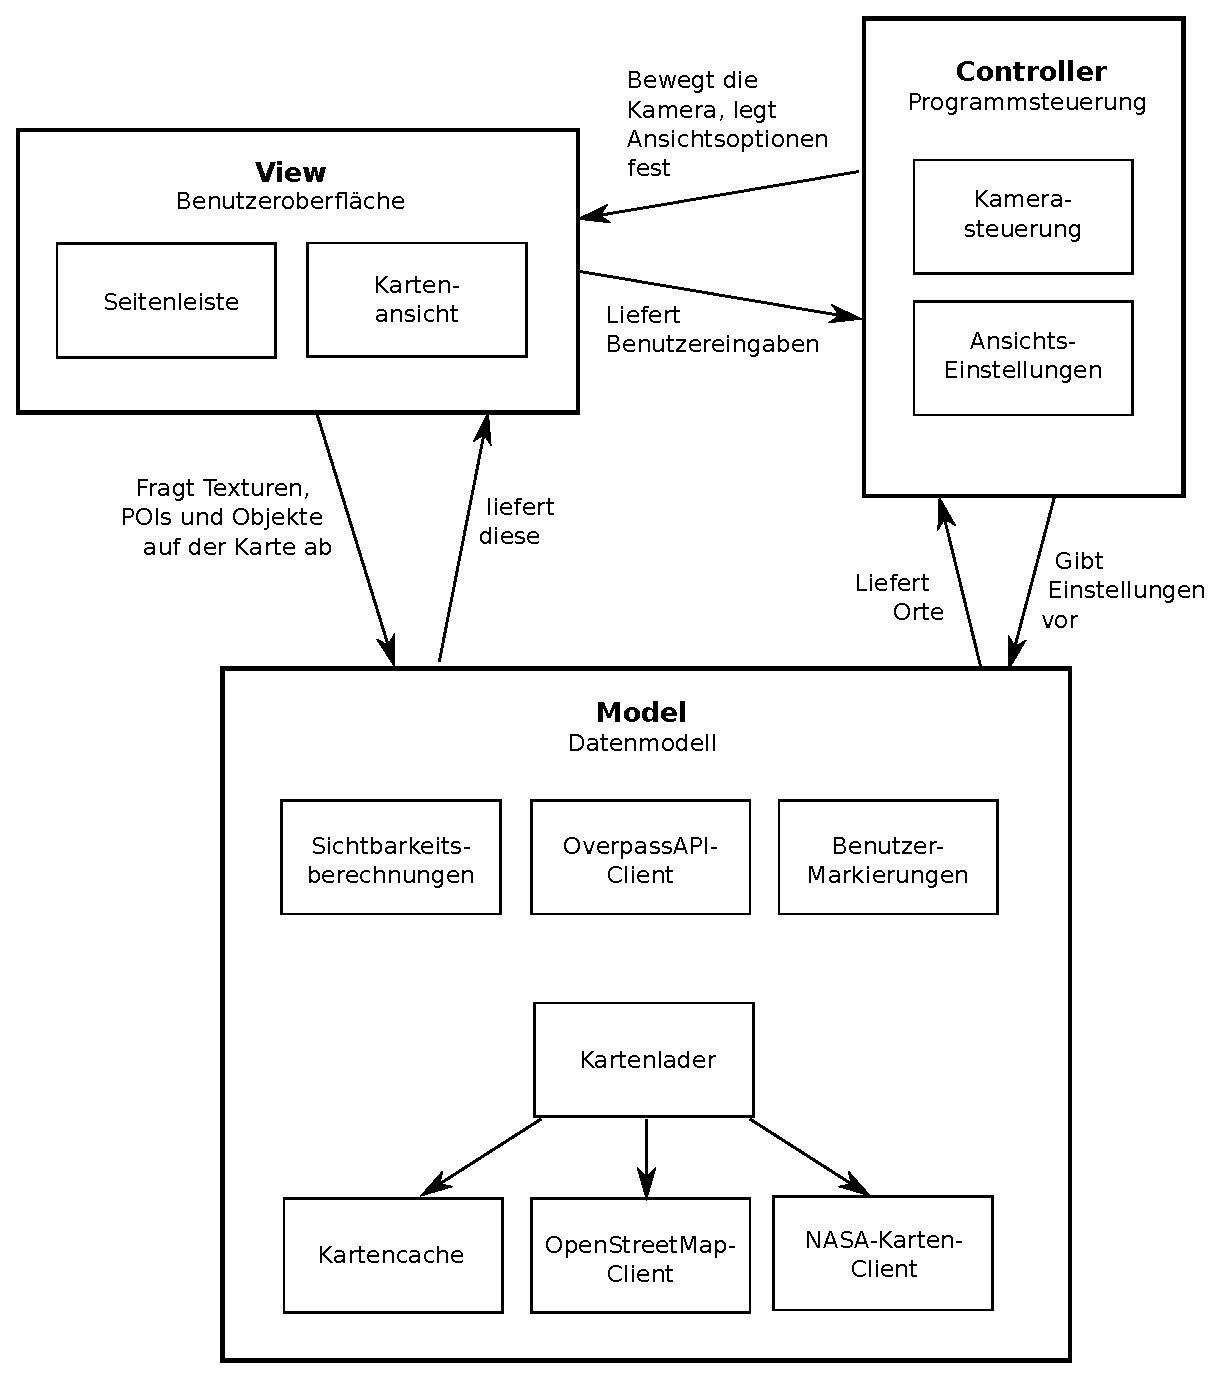
\includegraphics[scale=0.6]{ModelViewController.eps}
\caption{Die Systemarchitektur}
\end{figure}
\pagebreak
\subsection*{Controller}
Programmsteuerung
\begin{itemize}
\item Kamerasteuerung
\item Ansichtseinstellungen
\end{itemize}
\subsection*{View}
Benutzeroberfläche
\begin{itemize}
\item 3D-Ansicht
\item Seitenleiste
\end{itemize}
\subsection*{Model}
\begin{itemize}
\item Sichtbarkeitsberechnungen
\item OverpassAPI-Client
\item Benutzermarkierungen
\item \begin{itemize}
\item Kartencache
\item OpenStreetMap-Client
\item NASA-Karten-Client
\end{itemize}
\end{itemize}
\vspace{1cm}(Ausformulieren!)


\chapter{Produktfunktionen}

\nplpadding{2}
\renewcommand{\labelenumi}{\textbf{/F\numprint{\theenumi}0/}}

\newcommand{\W}{\textbf{W }}
Wunschkriterien werden mit \W  gekennzeichnet, alle verbleibenden sind Musskriterien.

\section{Fensterverhalten}
\begin{enumerate}[leftmargin=2cm]
\item Das Programmfenster startet mit einer Größe von 1024x768 Pixeln. Die Größe ist mit 800x600 Pixeln nach unten, aber nicht nach oben beschränkt und kann vom Benutzer beliebig  verändert werden.
\item \W Die Anwendung bietet einen Vollbildmodus, in dem Kartenansicht mit Seitenleiste über den gesamten Bildschirm gestreckt werden und Fensterdekorationen entfallen. Zwischen Fenster- und Vollbildmodus kann mit dem Tastenkürzel F11 gewechselt werden.
\item Mit dem Tastenkürzel Strg+Q wird die Anwendung ohne Rückfrage beendet.
\item \W Die Einstellungsleiste am linken Rand der GUI ist einklappbar.
\end{enumerate}
\section{Kartenansicht}
\begin{enumerate}[leftmargin=2cm,resume]
\item Die Kartenansicht kann interaktiv mit Maus oder Tastatur bedient werden.
\item \W Im Sonnensystemmodus HIER FEHLT WAS
\item Im 2D-Kartenmodus kann die Ansicht nach links/rechts und oben/unten verschoben sowie (perspektivisch) gekippt werden. 
\item Im 3D-Kartenmodus kann die Ansicht kann um die Erdachse sowie in Richtung der Pole gedreht; ab einem gewissen Zoomlevel am Kameraursprung gekippt werden.
\item Mit Linksklick-Ziehen oder den Pfeiltasten der Tastatur wird die Karte verschoben bzw. der Globus gedreht, mit Rechsklick-Ziehen nach oben/unten oder den BildAuf/BildAb-Tasten der Tastatur wird die Ansicht gekippt.
\item \W Mit einem einfachen Linksklick werden im Detailfenster zusätzliche Daten zum Punkt unter dem Mauszeiger angezeigt. Bei POIs sind das Adresse sowie Beschreibung; bei anderen Punkten genauer Längen- und Breitengrad.
\end{enumerate}
\section{Navigationsdaten}
\begin{enumerate}[leftmargin=2cm,resume]
\item Das Zoomlevel kann über einen Schieber angezeigt und geändert werden.
\item Der Längen- und Breitengrad des Punktes an der Bildschirmmitte wird über Eingabefelder angezeigt, und kann über sie geändert werden.
\item Ein Ladebalken zeigt den Fortschritt eventuell im Hintergrund geladener Kartendaten an.
\item Der Maßstab des Punktes unter dem Anzeigemittelpunkt wird in einem Feld angezeigt.
\end{enumerate}

\section{Ansichtseinstellungen}
\begin{enumerate}[leftmargin=2cm,resume]
\item Es kann zwischen 3D- (Globus) und 2D-Ansicht (Aufsicht) gewählt werden.
\item Es besteht eine Auswahl aus verschiedenen Kartentypen; wie Satellitenbildern und Straßenkarten.
\item \W Wird als Kartentyp die Kinder-Weltkarte gewählt, wir eine Auswahl an angezeigten POIs vorgegeben.
\item \W Es sind Höhenprofile, -linien, sowie 3D-Ansichten von Häusern und 
Bäumen zuschaltbar.
\end{enumerate}

\section{Orte}
\begin{enumerate}[leftmargin=2cm,resume]
\item Städtenamen, Points of Interest und andere Informationen können unter einer Vielzahl an Overlays an- und abgewählt werden.
\item \W Eigene Punkte können auf der Karte markiert, die Markierungen ein-/ausgeblendet, in einer Liste verwaltet und wieder entfernt werden.
\item \W Orte und POIs können mittels einer Suchfunktion aufgefunden, angezeigt und den markierten Punkten hinzugefügt werden. Es kann dabei entweder im momentanen Kartenausschnitt oder global gesucht werden.
\end{enumerate}

\section{Detailfenster}
\begin{enumerate}[leftmargin=2cm,resume]
\item Das Detailfenster bietet die Möglichkeit nähere Informationen zu einem Punkt auf der Karte zu erhalten, wie zugehörigem Längen- und Breitengrad. Des weiteren kann der Punkt markiert und gespeichert werden.
\end{enumerate}



\chapter{Produktdaten}

\renewcommand{\labelenumi}{\textbf{/D\numprint{\theenumi}0/}}
Wunschkriterien werden mit \W  gekennzeichnet, alle verbleibenden sind Musskriterien.

\section{Kartenansicht}
\begin{enumerate}[leftmargin=2cm]
\item Verfügbare Kartentypen sind:
\begin{itemize}
\item Satellitenbild
\item OpenStreetMap - Straßenkarte (Tag)
\item \W OpenStreetMap - Straßenkarte (Nacht)
\item \W Kinder - Weltkarte
\end{itemize}
\item Wählbare Overlays sind:
\begin{itemize}
\item Städte- und Ländernamen
\item Points of Interest, wie Banken, Tankstellen, Tierparks, Spielplätze etc.
\item Straßennamen
\item \W Länder- und Staatsgrenzen
\end{itemize}
\item \W In der 3D-Ansicht ist ein Sternenhimmel als Hintergrund zuschaltbar
\end{enumerate}

\section{Kartendaten}
\begin{enumerate}[leftmargin=2cm,resume]
\item Heruntergeladene Kacheln werden primär im Arbeitsspeicher (\W) und sekundär in einem Cache im temporären Verzeichnis des Betriebssystems zwischengespeichert.
\item Die Größe der Caches ist einstellbar. Standardmäßig ist der Cache im Arbeitsspeicher 50 MB, der im Dateisystem 200 MB groß.
\end{enumerate}

\section{GUI}
\begin{enumerate}[leftmargin=2cm,resume]
\item Oberfläche der GUI in Übersetzung: Englisch und Deutsch
\end{enumerate}


\chapter{Produktleistungen}

\renewcommand{\labelenumi}{\textbf{/L\numprint{\theenumi}0/}}
Wunschkriterien werden mit \W  gekennzeichnet, alle verbleibenden sind Musskriterien.

\section{Darstellung der Kartenansicht}
\begin{enumerate}[leftmargin=2cm]
\item Aus der aktuellen Perspektive werden die sichtbaren Kartenabschnitte und die nötige Kartenauflösung bestimmt.
\item Das Kartenmaterial ist in Kacheln aufgeteilt, die als Textur auf den Globus bzw. die Karte gelegt werden. Welche Kacheln geladen werden müssen, wird  aus den sichtbaren Kartenabschnitten und dem momentanen Zoomlevel bestimmt.
\item In 3D-Darstellung kann die Ansicht nicht über die Pole hinweg gedreht werden, sodass die Pole im Fenster immer nach oben oder unten zeigen.
\item Overlays wie Städtenamen oder Symbole für Tankstellen werden als zweidimensionale Objekte an die Stelle der Anzeigefläche projiziert, an der der markierte Punkt auf dem Bildschirm erscheint.
\item \W Dreidimensionale Objekte wie Häusermodelle, Bäume, oder Stecknadeln zur Markierung von Punkten werden direkt in die Szene eingefügt.
\end{enumerate}

\section{Laden der Kartendaten}
\begin{enumerate}[resume,leftmargin=2cm]
\item Ist die Textur einer Kachel bereits geladen, wird sie direkt zur Anzeige verwendet.
\item \W Ansonsten wird zuerst versucht sie aus dem Cache im Arbeitsspeicher, dann aus dem Cache im Dateisystem zu laden.
\item Ist sie lokal nicht vorhanden, wird sie über einen passenden Kachelserver nachgeladen und dem Cache hinzugefügt. Des weiteren können sogar die Server angepasst bzw. erweitert werden. Es werden nur die benötigen Karten für den jeweiligen Ausschnitt geladen sowie die direkten Randbereiche außerhalb der Ansicht (\W).
\item Ist eine Textur noch nicht geladen oder nicht verfügbar, wird sie zwischenzeitlich durch eine Platzhaltertextur ersetzt.
\item Das Laden von Kacheldaten erfolgt im Hintergrund, während die Ansicht weiter gerendert werden kann.
\item Das Laden von Kacheln geschieht über HTTP.
\end{enumerate}

\section{Qualitätsmerkmale}

\begin{enumerate}[leftmargin=2cm,resume]
\item Kartendaten werden effizient zwischengespeichert, um sowohl unnötiges Nachladen als auch den Speicherverbrauch zu minimieren.
\item \W Der Energieverbrauch wird durch das vermeiden unnötiger Renderzyklen minimiert.
\item \W Die Anwendung ist intuitiv mit der Toucheingabe auf Windows 8 bedienbar.
\item \W Die Grafikeinstellungen lassen sich anpassen, sodass die Leistung auch auf älterer Hardware akzeptabel ist.
\item Hintergrundvorgänge des Programms wie das Nachladen von Kartendaten unterbrechen den Rendervorgang nicht.
\item Schlägt das Laden einer Kachel vom Server oder das Übergeben einer Textur an OpenGL fehl, fährt das Programm ohne Unterbrechung unter Verwendung einer Ersatztextur fort.
\item Die Bewegung der Kamera und das anpassen des Zoomlevels wird derart beschränkt, dass keine Darstellungsfehler wie das Durchdringen der Kartenebene auftreten.
\item \W Die Menge der Angezeigten Overlays und 3D-Modelle wird beschränkt, sodass die Leistung wie auch die Lesbarkeit von Beschriftungen akzeptabel bleibt.
\end{enumerate}




\chapter{Benutzeroberfläche}

\begin{itemize}
	\item Das Hauptelement der Benutzeroberfläche ist die Karten- oder Globusansicht, die sich im rechten Fensterteil befindet. Der sichtbare Kartenausschnitt kann interaktiv mit Maus oder Tastatur verschoben werden.
	\item Im 2D-Modus zeigt die Ansicht eine Projektion der Karte auf die Ebene, die in der Ansicht nach links/rechts und oben/unten verschoben sowie (perspektivisch) gekippt werden kann.
	\item Im 3D-Modus wird ein Globus gezeigt, auf den das Kartenmaterial projiziert wird. Die Ansicht kann um die Erdachse sowie in Richtung der Pole gedreht; ab einem gewissen Zoomlevel am Kameraursprung gekippt werden.
	\item Am linken Rand des Fensters befindet sich eine Seitenleiste, die sämtliche Steuerungsfunktionen bereitstellt. Der obere Teil ist in Tabs unterteilt, mit denen Funktionen gruppiert werden; der untere Teil zeigt Details zum momentan Zentrierten Punkt an.
\end{itemize}


\begin{figure}
	\centering
	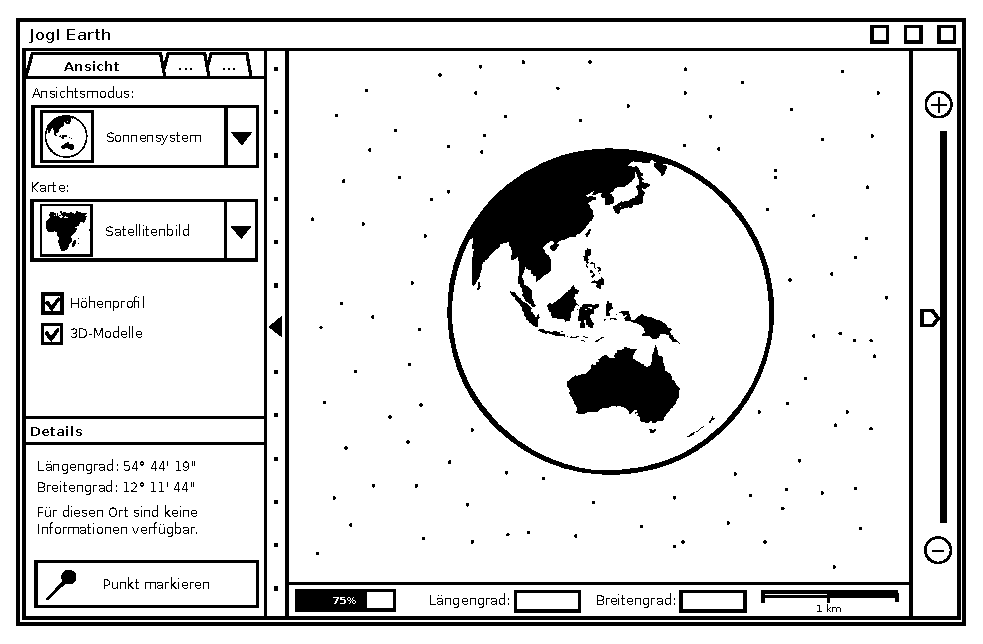
\includegraphics[scale=0.9]{GUI-Ansicht.eps}
	\caption{Die Benutzeroberfläche mit geöffnetem Ansichts-Tab}
\end{figure}
\begin{figure}
	\centering
	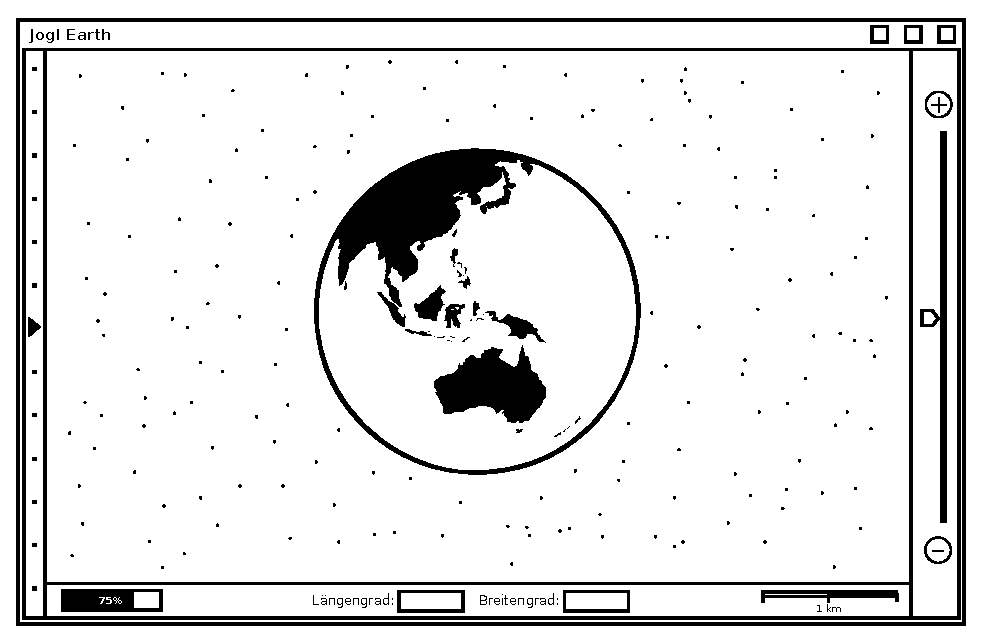
\includegraphics[scale=0.9]{GUI-Ausgeblendet.eps}
	\caption{Die Benutzeroberfläche mit ausgeblendeter Seitenleiste}
\end{figure}
\begin{figure}
	\centering
	\begin{minipage}[c]{6cm}
	\centering
		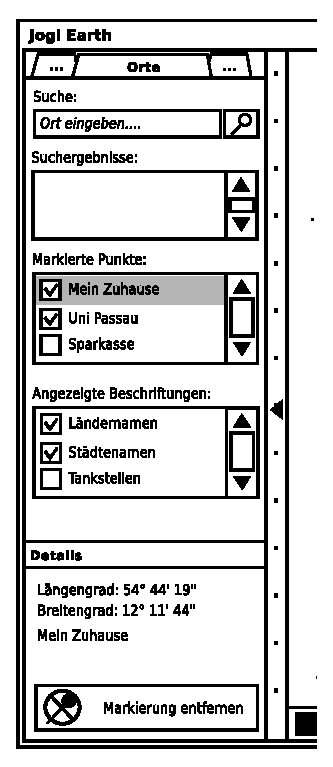
\includegraphics[scale=0.9]{GUI-Orte.eps}
	\end{minipage}
	\begin{minipage}[c]{6cm}
	\centering
		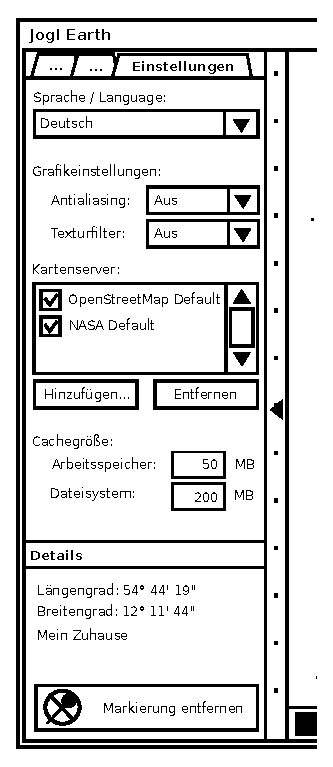
\includegraphics[scale=0.9]{GUI-Einstellungen.eps}
	\end{minipage}
	\caption{Der Orte- und der Einstellungstab}
\end{figure}
\begin{figure}
	\centering
	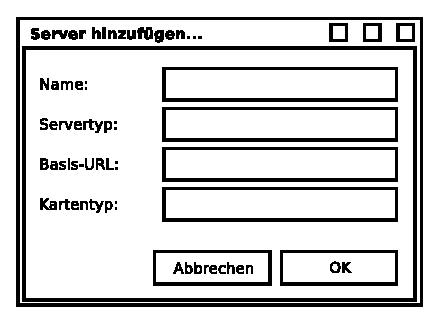
\includegraphics[scale=0.9]{GUI-ServerDialog.eps}
	\caption{Das Dialogfenster zum Hinzufügen eines neuen Servers}
\end{figure}




\chapter{Qualitätsbestimmungen}

\section{Funktionalität}
\begin{itemize}
\item Web Mining: Automatische Extraktion von Daten aus dem Internet. Bei \"Jogl Earth" findet das Web Mining bei der Suchfunktion z.B. nach Orten Anwendung.
\item Interoperabilität: Das Programm \"Jogl Earth" soll mit OpenStreetMap und der Overpass-API und Ähnlichen Diensten interagieren um das Kartenmaterial mit Zusatzinformationen grafisch zu unterstützen.
\end{itemize}


\section{Zuverlässigkeit}
\begin{itemize}
\item Stabilität: Die Lauffähigkeit des Programms soll nicht unterbrochen bzw. beeinträchtigt werden.
\item Fehlertoleranz: Das Programm soll trotz fehlerhafter Eingaben seine Funktionsweise aufrechterhalten.
\item Wiederherstellbarkeit: Das Programm soll nach Beendigung wieder im gleichen Zustand verfügbar sein.
\end{itemize}


\section{Benutzbarkeit}
\begin{itemize}
\item Bedienbarkeit: Die Oberfläche soll intuitiv bedienbar sein.
\item Erlernbarkeit: Die Bedienung der Oberfläche soll einfach verstanden werden.
\item Grafische Gestaltung: Die Oberfläche soll optisch ansprechend wirken.
\item Verständlichkeit: Die Oberfläche soll selbsterklärend sein.
\end{itemize}


\section{Effizienz}
\begin{itemize}
\item Bildqualität: Die Satellitenbilder und Kartendaten sollen in bestmöglicher Qualität dargestellt werden.
\item Laufzeit: Trotz bestmöglicher Bildqualität sollen die Wartezeiten zum Laden der Daten gering gehalten werden.
\item Speichermanagement: Die Kachel-Daten werden im Dateisystem und im Arbeitsspeicher effizient gepuffert.
\end{itemize}


\section{Anpassfähigkeit}
\begin{itemize}
\item Code-Qualität: Der Quellcode des Programms soll leicht verständlich gehalten werden.
\item Modifizierbarkeit: Zusätzliche Änderungen bzw. Anpassungen des Codes sollen einfach umsetzbar sein.
\end{itemize}


\section{Portierbarkeit}
\begin{itemize}
\item Erweiterbarkeit: Zusätzliche Funktionalitäten sollen in den Code integrierbar sein.
\item Konformität: Vorgegebene Konventionen sollen eingehalten werden.
\end{itemize}


\section{Dokumentation}
Das Benutzerhandbuch, die Javadocs, die einzelnen Phasendokumente usw. sollen gut strukturiert, leicht verständlich, fachlich kompetent gehalten sein. 


\section{Bewertung der Qualitätsbestimmungen}
\begin{center}
\begin{tabular}{lcccc}
\hline 
\rule[-1ex]{0pt}{4ex} \textit{Produktqualität} & \textit{sehr gut} & \textit{gut} & \textit{normal} & \textit{nicht relevant} \\ 
\hline 
\rule[-1ex]{0pt}{4ex} \textbf{Funktionalität} &  &  &  &  \\ 
\rule[-1ex]{0pt}{4ex} \hspace{10pt} Güte Web Mining & &  & • & \\ 
\rule[-1ex]{0pt}{4ex} \hspace{10pt} Interoperabilität & & • & & \\ 

\hline 
\rule[-1ex]{0pt}{4ex} \textbf{Zuverlässigkeit} &  &  &  &  \\ 
\rule[-1ex]{0pt}{4ex} \hspace{10pt} Stabilität & • & & & \\ 
\rule[-1ex]{0pt}{4ex} \hspace{10pt} Fehlertoleranz & • & & & \\ 
\rule[-1ex]{0pt}{4ex} \hspace{10pt} Wiederherstellbarkeit &  &  &  & • \\ 

\hline 
\rule[-1ex]{0pt}{4ex} \textbf{Benutzbarkeit} &  &  &  &  \\ 
\rule[-1ex]{0pt}{4ex} \hspace{10pt} Bedienbarkeit & • & & & \\ 
\rule[-1ex]{0pt}{4ex} \hspace{10pt} Erlernbarkeit & • & & & \\ 
\rule[-1ex]{0pt}{4ex} \hspace{10pt} Grafische Gestaltung & & • & & \\ 
\rule[-1ex]{0pt}{4ex} \hspace{10pt} Verständlichkeit & • & & & \\ 

\hline 
\rule[-1ex]{0pt}{4ex} \textbf{Effizienz} &  &  &  &  \\ 
\rule[-1ex]{0pt}{4ex} \hspace{10pt} Bildqualität & & • & & \\ 
\rule[-1ex]{0pt}{4ex} \hspace{10pt} Laufzeit & & • & & \\ 
\rule[-1ex]{0pt}{4ex} \hspace{10pt} Speichermanagement & • & & & \\ 

\hline 
\rule[-1ex]{0pt}{4ex} \textbf{Anpassfähigkeit} &  &  &  &  \\ 
\rule[-1ex]{0pt}{4ex} \hspace{10pt} Code-Qualität & & • & & \\ 
\rule[-1ex]{0pt}{4ex} \hspace{10pt} Modifizierbarkeit & & & • & \\ 

\hline 
\rule[-1ex]{0pt}{4ex} \textbf{Portierbarkeit} &  &  &  &  \\ 
\rule[-1ex]{0pt}{4ex} \hspace{10pt} Erweiterbarkeit & & & • & \\ 
\rule[-1ex]{0pt}{4ex} \hspace{10pt} Konformität & & • & & \\ 

\hline 
\rule[-1ex]{0pt}{4ex} \textbf{Dokumentation} & • & & & \\ 
\hline 
\end{tabular} 
\end{center}




\chapter{Globale Testszenarien und Testfälle}





\chapter{Entwicklungsumgebung}
\section{Software}
Abgesehen vom Betriebssystem und Anwendungen wie Texteditoren ist die verwendete Software im Entwicklerteam einheitlich.
\begin{itemize}
\item Betriebssysteme: Windows 7, Windows 8, Linux, jeweils auf x86{\_}64
\item Entwicklungsumgebung: Eclipse
\item Framework: Java 7 (JDK)
\item Textsatz: \LaTeX
\item Versionsverwaltung: Git
\item Visualisierung: IBM Software Rational Architect
\end{itemize}


\section{Hardware}
Auch wenn die Hardwareanforderungen bereits gegeben sind, sei hier einmal die Ausstattung der Entwickler aufgeführt um die genauen Testbedingungen zu formulieren.

\vspace{0.5cm}

\begin{tabular}{l|c|c|c}
\textsf{\textbf{Entwickler}} & \textsf{\textbf{Prozessor}} & \textsf{\textbf{RAM}} & \textsf{\textbf{Grafik}} \\
Fabian Knorr & AMD PhenomII X4 840 @3,2GHz & 8 GB & ATi Radeon HD 6850 \\
Fabian Knorr & AMD Athlon Neo X2 L335 @1,6GHz & 4 GB & ATi Radeon HD 3200 \\
Gabriele Haas & Intel Core i3 550 @3,2GHz & 4 GB & Intel HD Graphics (i3) \\
Christof Blauberger & AMD A6-3420M & 8 GB & ATi Radeon HD 6520/7470M \\
Constantin Wenger & Intel i7-3770K @3.50GHz & 24GB & Nvidia GTX 770 4GB \\
Thomas Eder & AMD A4-3400 & 8 GB & Nvidia GTX 260 \\
Sebastian Reichl & AMD PhenomII X6 1100T @3,4Ghz & 8 GB & ATI Radeon HD 6950 \\
Sebastian Reichl & Intel Core i5-4200U @ 2,29 Ghz & 4 GB & Intel HD Graphics \\
\end{tabular}

\vspace{0.5cm}



\chapter{Anhang}
\section{Glossar}
\newcolumntype{L}[1]{>{\sffamily\bfseries\hsize=#1\hsize\raggedright\arraybackslash}X}
\newcolumntype{R}[1]{>{\hsize=#1\hsize\raggedright\arraybackslash}X}
\setlength{\extrarowheight}{3mm}
\begin{tabularx}{\textwidth}{L{0.35} R{1.65}}
Anisotropes Filtern & Methode um den Schärfeeindruck von perspektivisch deformierten Texturen zu erhalten\\
Antialiasing & Methode zur Kantenglättung in Grafiken\\
API & Application Programming Interface, englische Bezeichnung für Anwendungsschnittstelle\\
Detailfenster & Zeigt alle Details zu einem markierten Punkt [Streichen?]\\
Eclipse & Software-Plattform und Integrierte Entwicklungsumgebung für (u.a.) Java\\
Git & Verteiltes Versionsverwaltungssystem\\
Java & Programmiersprache, siehe auch: JRE\\
Javadoc & Dokumentation von Klassen und Methoden in Java\\
JOGL & (Java OpenGL) Softwarebibliothek, die die OpenGL-API in Java zur Verfügung stellt\\
{\LaTeX} & Freies Textsatzprogramm für wissenschaftliche Arbeiten\\
OpenGL & API zur Generierung von 2D- und 3D-Computergrafik\\
OpenStreetMap & Projekt, das freies Kartenmaterial im Internet anbietet\\
Overlay & Text- oder Symboleinblendungen auf den Karten bzw. der Weltkugel\\
Plattform"-unabhängigkeit & Das Programm kann auf mehreren Betriebssystemen ausgeführt werden ohne Anpassungen zu erfordern.\\
POI & (Point Of Interest) POIs sind Orte auf der Weltkarte, die eine spezielle Bedeutung haben, wie Tankstellen, Banken, Tierparks oder Sehenswürdigkeiten.\\
RAM & (Random Access Memory) Arbeitsspeicher.\\
Rendern & Erzeugen eines Bildes aus Rohdaten, hier aus einem räumlichen Modell\\
Server & Gegenstelle im Netzwerk, die einen Dienst zur Verfügung stellt, hier Lieferung des Kartenmaterials\\
Textur & Zweidimensionale (Oberflächen-) Grafik im Kontext von Rendern.\\
\end{tabularx}



\end {document}
